% Options for packages loaded elsewhere
\PassOptionsToPackage{unicode}{hyperref}
\PassOptionsToPackage{hyphens}{url}
%
\documentclass[
]{article}
\usepackage{amsmath,amssymb}
\usepackage{lmodern}
\usepackage{iftex}
\ifPDFTeX
  \usepackage[T1]{fontenc}
  \usepackage[utf8]{inputenc}
  \usepackage{textcomp} % provide euro and other symbols
\else % if luatex or xetex
  \usepackage{unicode-math}
  \defaultfontfeatures{Scale=MatchLowercase}
  \defaultfontfeatures[\rmfamily]{Ligatures=TeX,Scale=1}
\fi
% Use upquote if available, for straight quotes in verbatim environments
\IfFileExists{upquote.sty}{\usepackage{upquote}}{}
\IfFileExists{microtype.sty}{% use microtype if available
  \usepackage[]{microtype}
  \UseMicrotypeSet[protrusion]{basicmath} % disable protrusion for tt fonts
}{}
\makeatletter
\@ifundefined{KOMAClassName}{% if non-KOMA class
  \IfFileExists{parskip.sty}{%
    \usepackage{parskip}
  }{% else
    \setlength{\parindent}{0pt}
    \setlength{\parskip}{6pt plus 2pt minus 1pt}}
}{% if KOMA class
  \KOMAoptions{parskip=half}}
\makeatother
\usepackage{xcolor}
\usepackage[margin=1in]{geometry}
\usepackage{color}
\usepackage{fancyvrb}
\newcommand{\VerbBar}{|}
\newcommand{\VERB}{\Verb[commandchars=\\\{\}]}
\DefineVerbatimEnvironment{Highlighting}{Verbatim}{commandchars=\\\{\}}
% Add ',fontsize=\small' for more characters per line
\usepackage{framed}
\definecolor{shadecolor}{RGB}{248,248,248}
\newenvironment{Shaded}{\begin{snugshade}}{\end{snugshade}}
\newcommand{\AlertTok}[1]{\textcolor[rgb]{0.94,0.16,0.16}{#1}}
\newcommand{\AnnotationTok}[1]{\textcolor[rgb]{0.56,0.35,0.01}{\textbf{\textit{#1}}}}
\newcommand{\AttributeTok}[1]{\textcolor[rgb]{0.77,0.63,0.00}{#1}}
\newcommand{\BaseNTok}[1]{\textcolor[rgb]{0.00,0.00,0.81}{#1}}
\newcommand{\BuiltInTok}[1]{#1}
\newcommand{\CharTok}[1]{\textcolor[rgb]{0.31,0.60,0.02}{#1}}
\newcommand{\CommentTok}[1]{\textcolor[rgb]{0.56,0.35,0.01}{\textit{#1}}}
\newcommand{\CommentVarTok}[1]{\textcolor[rgb]{0.56,0.35,0.01}{\textbf{\textit{#1}}}}
\newcommand{\ConstantTok}[1]{\textcolor[rgb]{0.00,0.00,0.00}{#1}}
\newcommand{\ControlFlowTok}[1]{\textcolor[rgb]{0.13,0.29,0.53}{\textbf{#1}}}
\newcommand{\DataTypeTok}[1]{\textcolor[rgb]{0.13,0.29,0.53}{#1}}
\newcommand{\DecValTok}[1]{\textcolor[rgb]{0.00,0.00,0.81}{#1}}
\newcommand{\DocumentationTok}[1]{\textcolor[rgb]{0.56,0.35,0.01}{\textbf{\textit{#1}}}}
\newcommand{\ErrorTok}[1]{\textcolor[rgb]{0.64,0.00,0.00}{\textbf{#1}}}
\newcommand{\ExtensionTok}[1]{#1}
\newcommand{\FloatTok}[1]{\textcolor[rgb]{0.00,0.00,0.81}{#1}}
\newcommand{\FunctionTok}[1]{\textcolor[rgb]{0.00,0.00,0.00}{#1}}
\newcommand{\ImportTok}[1]{#1}
\newcommand{\InformationTok}[1]{\textcolor[rgb]{0.56,0.35,0.01}{\textbf{\textit{#1}}}}
\newcommand{\KeywordTok}[1]{\textcolor[rgb]{0.13,0.29,0.53}{\textbf{#1}}}
\newcommand{\NormalTok}[1]{#1}
\newcommand{\OperatorTok}[1]{\textcolor[rgb]{0.81,0.36,0.00}{\textbf{#1}}}
\newcommand{\OtherTok}[1]{\textcolor[rgb]{0.56,0.35,0.01}{#1}}
\newcommand{\PreprocessorTok}[1]{\textcolor[rgb]{0.56,0.35,0.01}{\textit{#1}}}
\newcommand{\RegionMarkerTok}[1]{#1}
\newcommand{\SpecialCharTok}[1]{\textcolor[rgb]{0.00,0.00,0.00}{#1}}
\newcommand{\SpecialStringTok}[1]{\textcolor[rgb]{0.31,0.60,0.02}{#1}}
\newcommand{\StringTok}[1]{\textcolor[rgb]{0.31,0.60,0.02}{#1}}
\newcommand{\VariableTok}[1]{\textcolor[rgb]{0.00,0.00,0.00}{#1}}
\newcommand{\VerbatimStringTok}[1]{\textcolor[rgb]{0.31,0.60,0.02}{#1}}
\newcommand{\WarningTok}[1]{\textcolor[rgb]{0.56,0.35,0.01}{\textbf{\textit{#1}}}}
\usepackage{graphicx}
\makeatletter
\def\maxwidth{\ifdim\Gin@nat@width>\linewidth\linewidth\else\Gin@nat@width\fi}
\def\maxheight{\ifdim\Gin@nat@height>\textheight\textheight\else\Gin@nat@height\fi}
\makeatother
% Scale images if necessary, so that they will not overflow the page
% margins by default, and it is still possible to overwrite the defaults
% using explicit options in \includegraphics[width, height, ...]{}
\setkeys{Gin}{width=\maxwidth,height=\maxheight,keepaspectratio}
% Set default figure placement to htbp
\makeatletter
\def\fps@figure{htbp}
\makeatother
\setlength{\emergencystretch}{3em} % prevent overfull lines
\providecommand{\tightlist}{%
  \setlength{\itemsep}{0pt}\setlength{\parskip}{0pt}}
\setcounter{secnumdepth}{-\maxdimen} % remove section numbering
\ifLuaTeX
  \usepackage{selnolig}  % disable illegal ligatures
\fi
\IfFileExists{bookmark.sty}{\usepackage{bookmark}}{\usepackage{hyperref}}
\IfFileExists{xurl.sty}{\usepackage{xurl}}{} % add URL line breaks if available
\urlstyle{same} % disable monospaced font for URLs
\hypersetup{
  pdftitle={Vaupés eBird},
  pdfauthor={Orlando Acevedo-Charry, et al.},
  hidelinks,
  pdfcreator={LaTeX via pandoc}}

\title{Vaupés eBird}
\author{Orlando Acevedo-Charry, et al.}
\date{2024-07-12}

\begin{document}
\maketitle

This code presents the analysis of eBird data from Mitú, Vaupés, in the
easternmost Amazon region of Colombia. The aim is to use eBird data to
evaluate community science contribution in a remote region of
northwestern Amazonia.

Este código presenta el análisis de los datos de eBird de Mitú, Vaupés,
en el borde oriental de la Amazonia colombiana. El objetivo es usar
datos de eBird para evaluarl la contribución de ciencia comunitaria en
una región remota de la Amazonia noroccidental.

\hypertarget{packages-needed---paquetes-necesarios}{%
\subsection{Packages needed - Paquetes
necesarios}\label{packages-needed---paquetes-necesarios}}

You will need to have some packages installed to access the data and
manipulate it.

Necesitara tener algunos paquetes instalados para accesar los datos y
manipularlos.

\begin{Shaded}
\begin{Highlighting}[]
\CommentTok{\#eBird data filters {-} filtro a los datos de eBird}
\FunctionTok{library}\NormalTok{(auk); }
\end{Highlighting}
\end{Shaded}

\begin{verbatim}
## auk 0.6.0 is designed for EBD files downloaded after 2022-10-25. 
## No EBD data directory set, see ?auk_set_ebd_path to set EBD_PATH 
## eBird taxonomy version:  2022
\end{verbatim}

\begin{Shaded}
\begin{Highlighting}[]
\CommentTok{\#seven packages in one for data management and visualization {-} siete paquetes en uno para manipulación y visualización de datos}
\FunctionTok{library}\NormalTok{(tidyverse);}
\end{Highlighting}
\end{Shaded}

\begin{verbatim}
## -- Attaching core tidyverse packages ------------------------ tidyverse 2.0.0 --
## v dplyr     1.1.4     v readr     2.1.5
## v forcats   1.0.0     v stringr   1.5.1
## v ggplot2   3.5.1     v tibble    3.2.1
## v lubridate 1.9.2     v tidyr     1.3.1
## v purrr     1.0.2
\end{verbatim}

\begin{verbatim}
## -- Conflicts ------------------------------------------ tidyverse_conflicts() --
## x dplyr::filter() masks stats::filter()
## x dplyr::lag()    masks stats::lag()
## i Use the conflicted package (<http://conflicted.r-lib.org/>) to force all conflicts to become errors
\end{verbatim}

\begin{Shaded}
\begin{Highlighting}[]
\CommentTok{\#Spatiotemporal Subsampling {-} submuestreo espaciotemporal}
\FunctionTok{library}\NormalTok{(dggridR); }
\end{Highlighting}
\end{Shaded}

\begin{verbatim}
## Loading required package: rlang
## 
## Attaching package: 'rlang'
## 
## The following objects are masked from 'package:purrr':
## 
##     %@%, flatten, flatten_chr, flatten_dbl, flatten_int, flatten_lgl,
##     flatten_raw, invoke, splice
## 
## Loading required package: sf
## Linking to GEOS 3.11.0, GDAL 3.5.3, PROJ 9.1.0; sf_use_s2() is TRUE
## Loading required package: sp
\end{verbatim}

\begin{Shaded}
\begin{Highlighting}[]
\CommentTok{\#load maps {-} cargar mapas}
\FunctionTok{library}\NormalTok{(maps); }
\end{Highlighting}
\end{Shaded}

\begin{verbatim}
## 
## Attaching package: 'maps'
## 
## The following object is masked from 'package:purrr':
## 
##     map
\end{verbatim}

\begin{Shaded}
\begin{Highlighting}[]
\CommentTok{\#composite figure {-} figuras compuestas}
\FunctionTok{library}\NormalTok{(gridExtra); }
\end{Highlighting}
\end{Shaded}

\begin{verbatim}
## 
## Attaching package: 'gridExtra'
## 
## The following object is masked from 'package:dplyr':
## 
##     combine
\end{verbatim}

\begin{Shaded}
\begin{Highlighting}[]
\CommentTok{\#Sankey plot with ggplot}
\FunctionTok{library}\NormalTok{(ggsankey) }\CommentTok{\#should be installed via \textasciigrave{}devtools::install\_github("davidsjoberg/ggsankey")\textasciigrave{}}
\end{Highlighting}
\end{Shaded}

\hypertarget{ebird-data-download---descarga-de-datos-de-ebird}{%
\subsection{1. eBird data download - descarga de datos de
eBird}\label{ebird-data-download---descarga-de-datos-de-ebird}}

We download the eBird data in
\href{https://ebird.org/data/download}{eBird - Data Access} - you should
be logged in.

Descargamos los datos de eBird en
\href{https://ebird.org/data/download}{eBird - Acceso a los datos} -
debe ingresar con su cuenta.

\begin{figure}
\centering
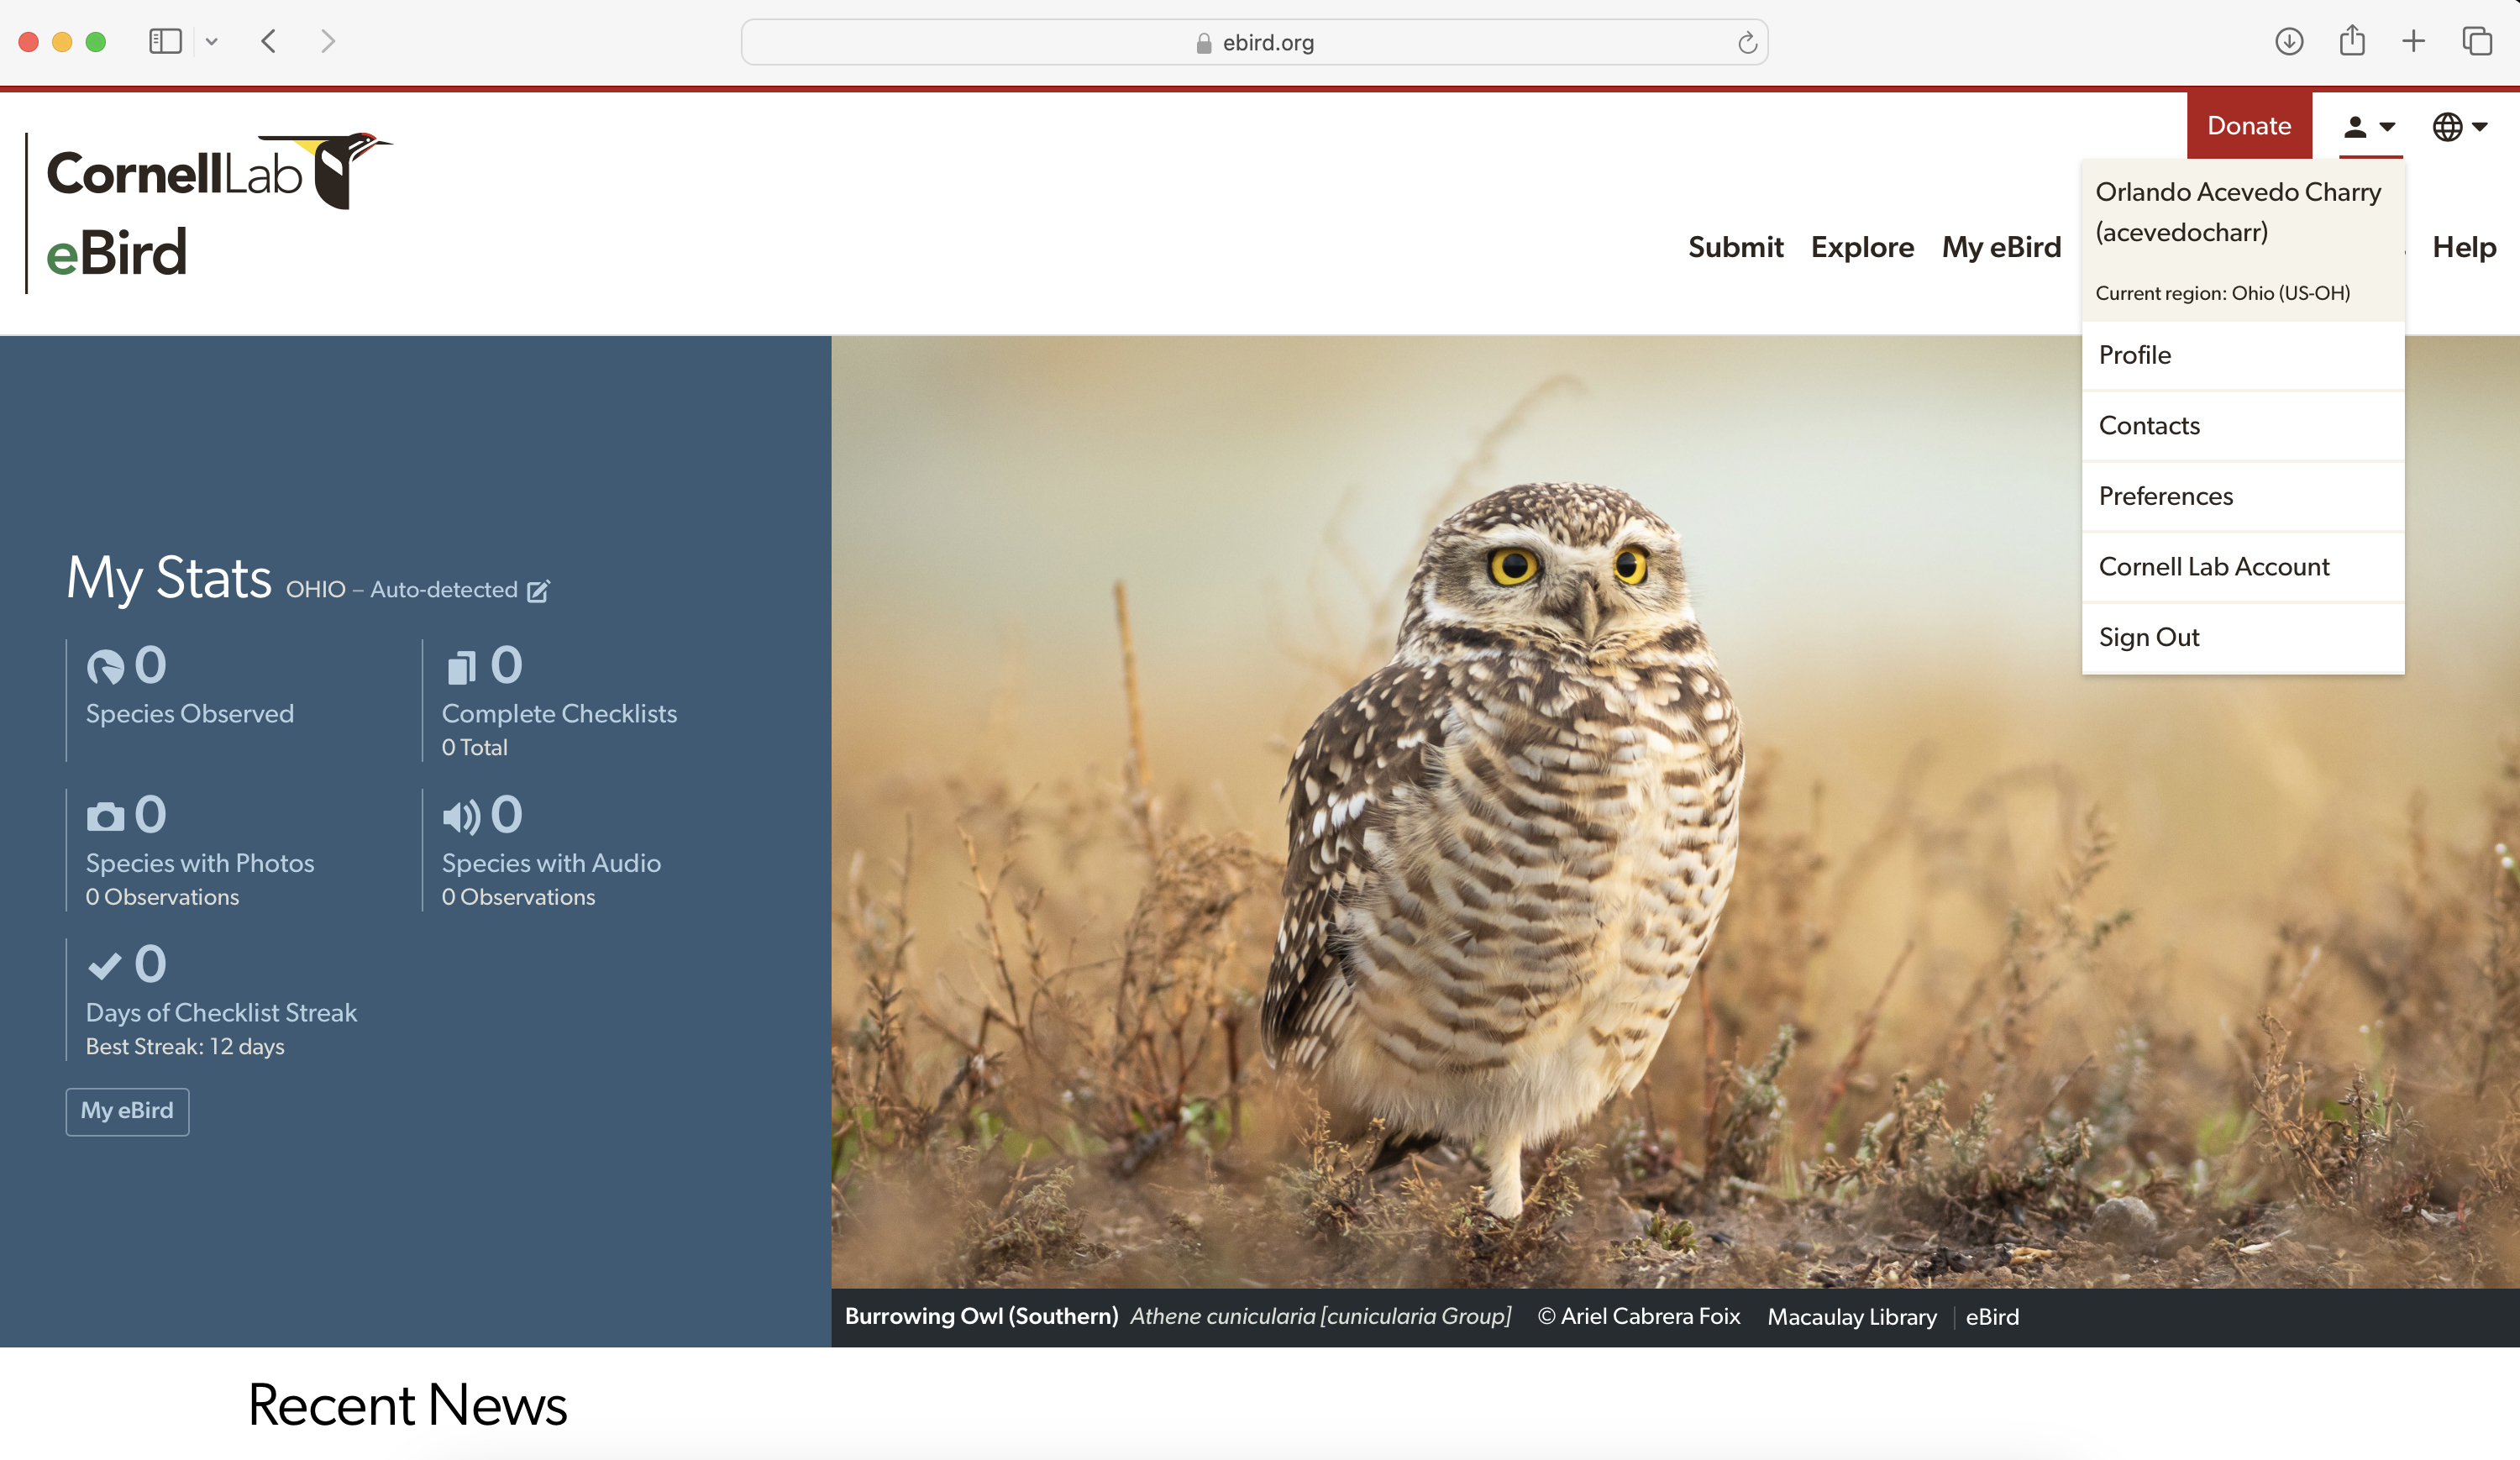
\includegraphics{screenshots/eBird1.png}
\caption{Go to eBird - vaya a eBird}
\end{figure}

Then, go to the bottom of the page, and click on ``Request data''

Vaya hasta la parte de abajo de la página y haga click en ``Pedir
datos''

\begin{figure}
\centering

\includegraphics{screenshots/eBird2.png}
\caption{to the bottom - hasta abajo}
\end{figure}

Click on ``Basic dataset (EBD)''

Seleccione el ``Conjunto de datos básico (EBD)''

\begin{figure}
\centering
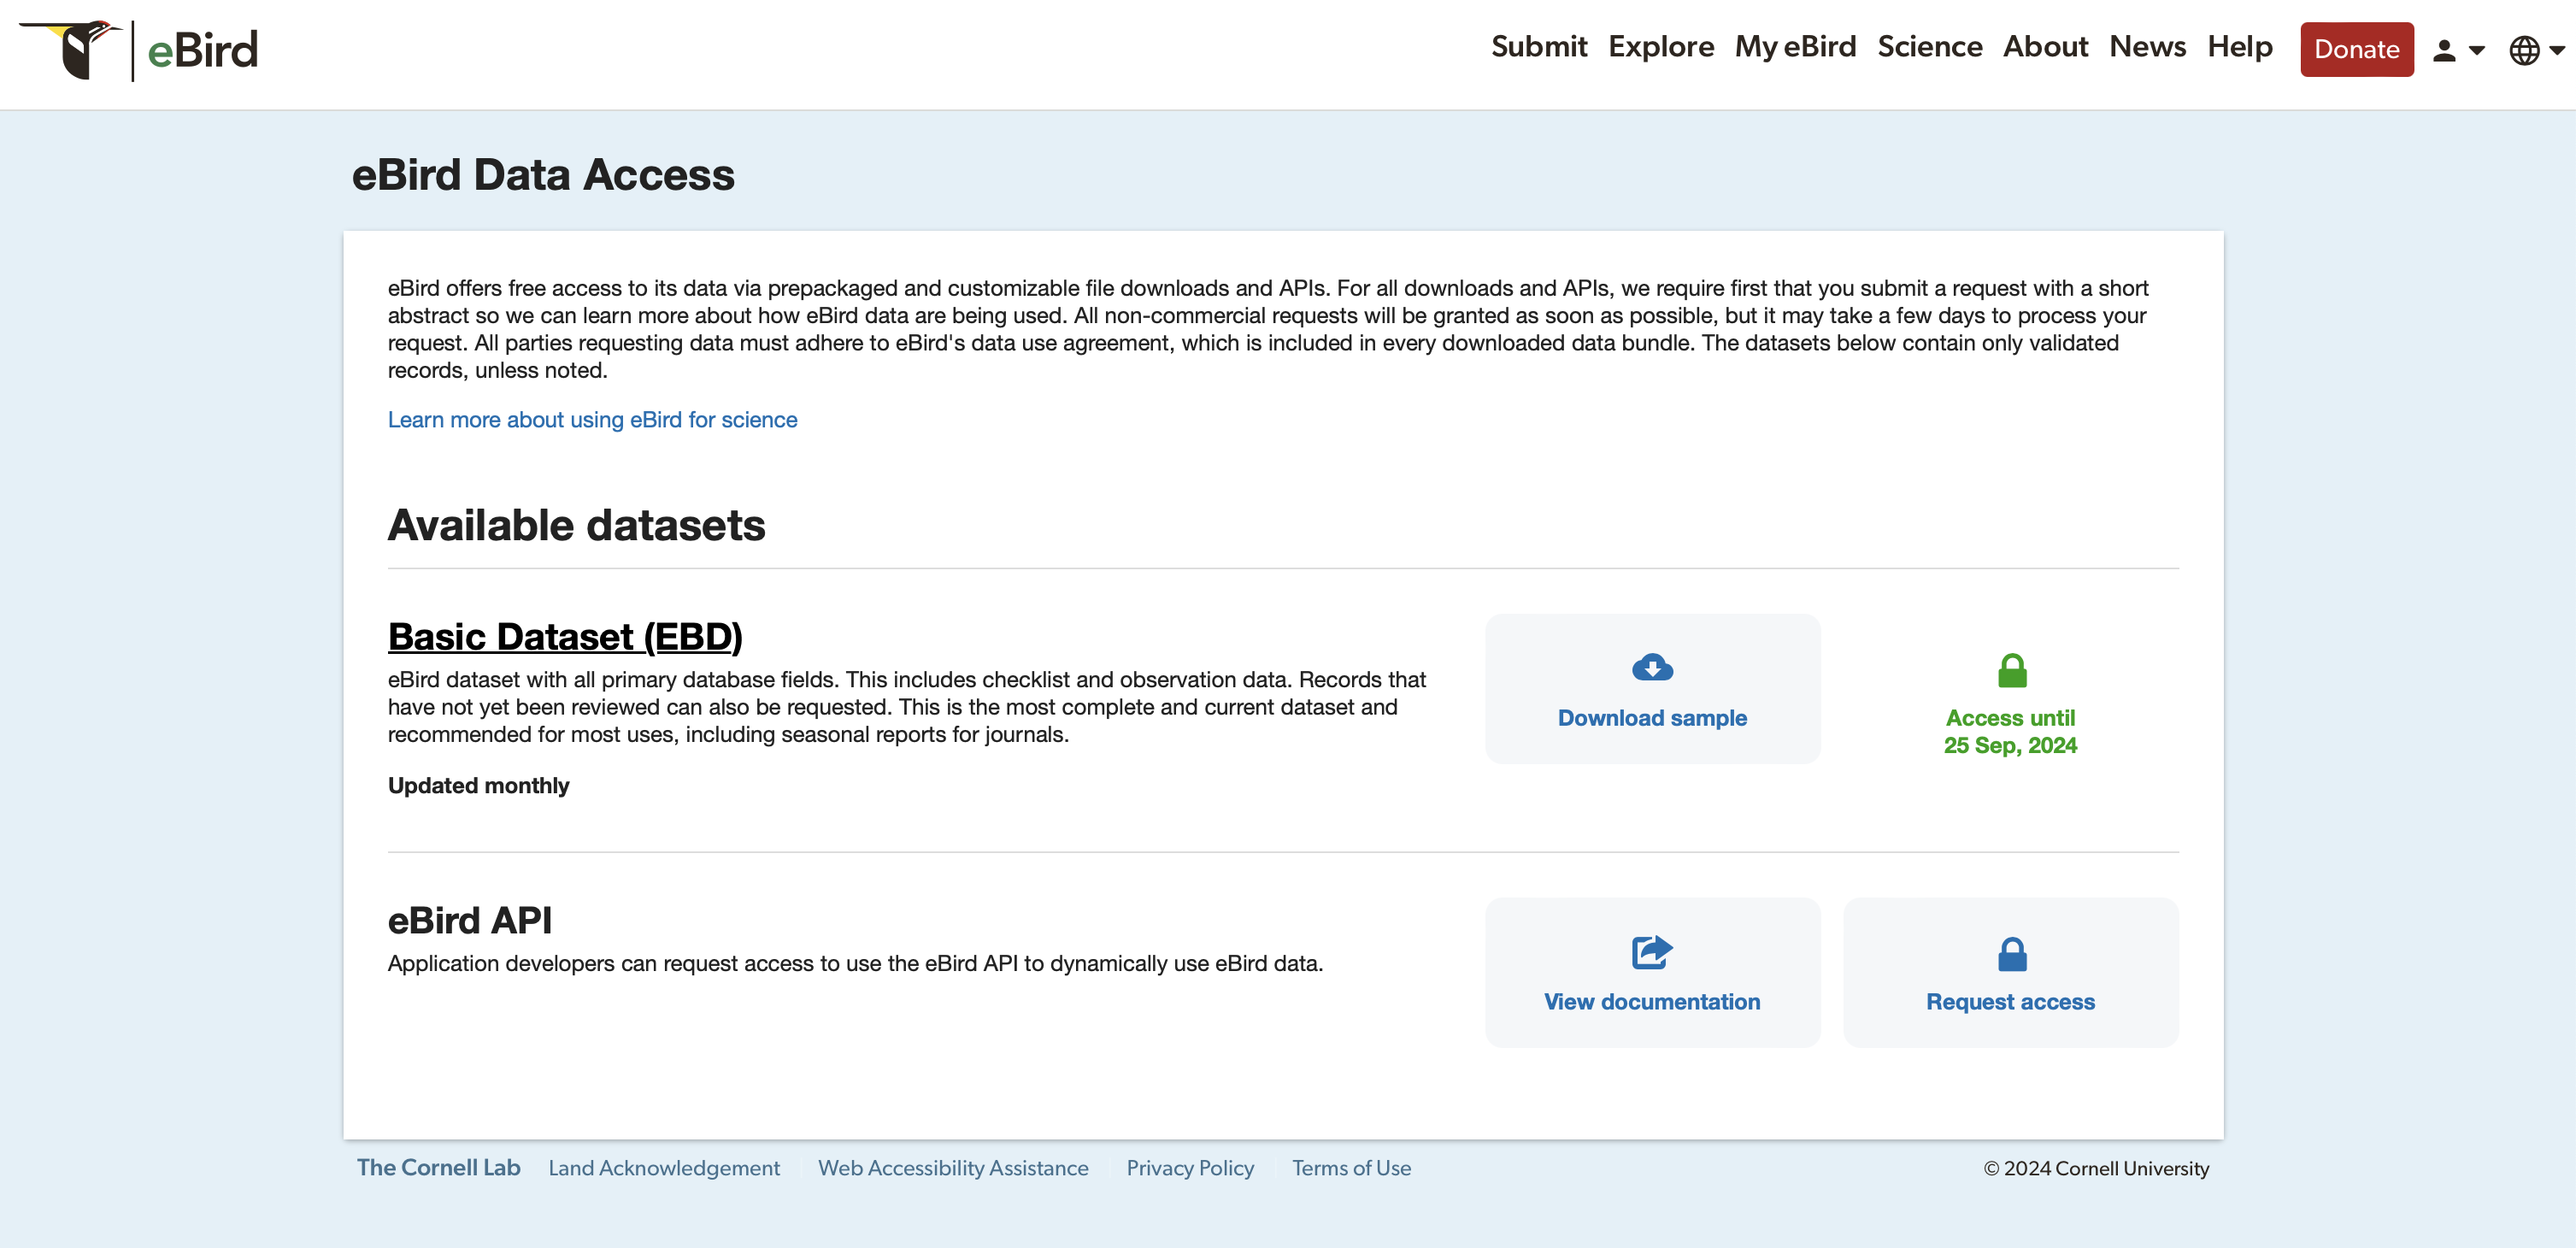
\includegraphics{screenshots/eBird3.png}
\caption{Basic ebd - ebd básico}
\end{figure}

And add the region, in our case \texttt{Vaupés,\ Colombia\ (CO)}

Y escriba la región, en nuestro caso \texttt{Vaupés,\ Colombia\ (CO)}

\begin{figure}
\centering
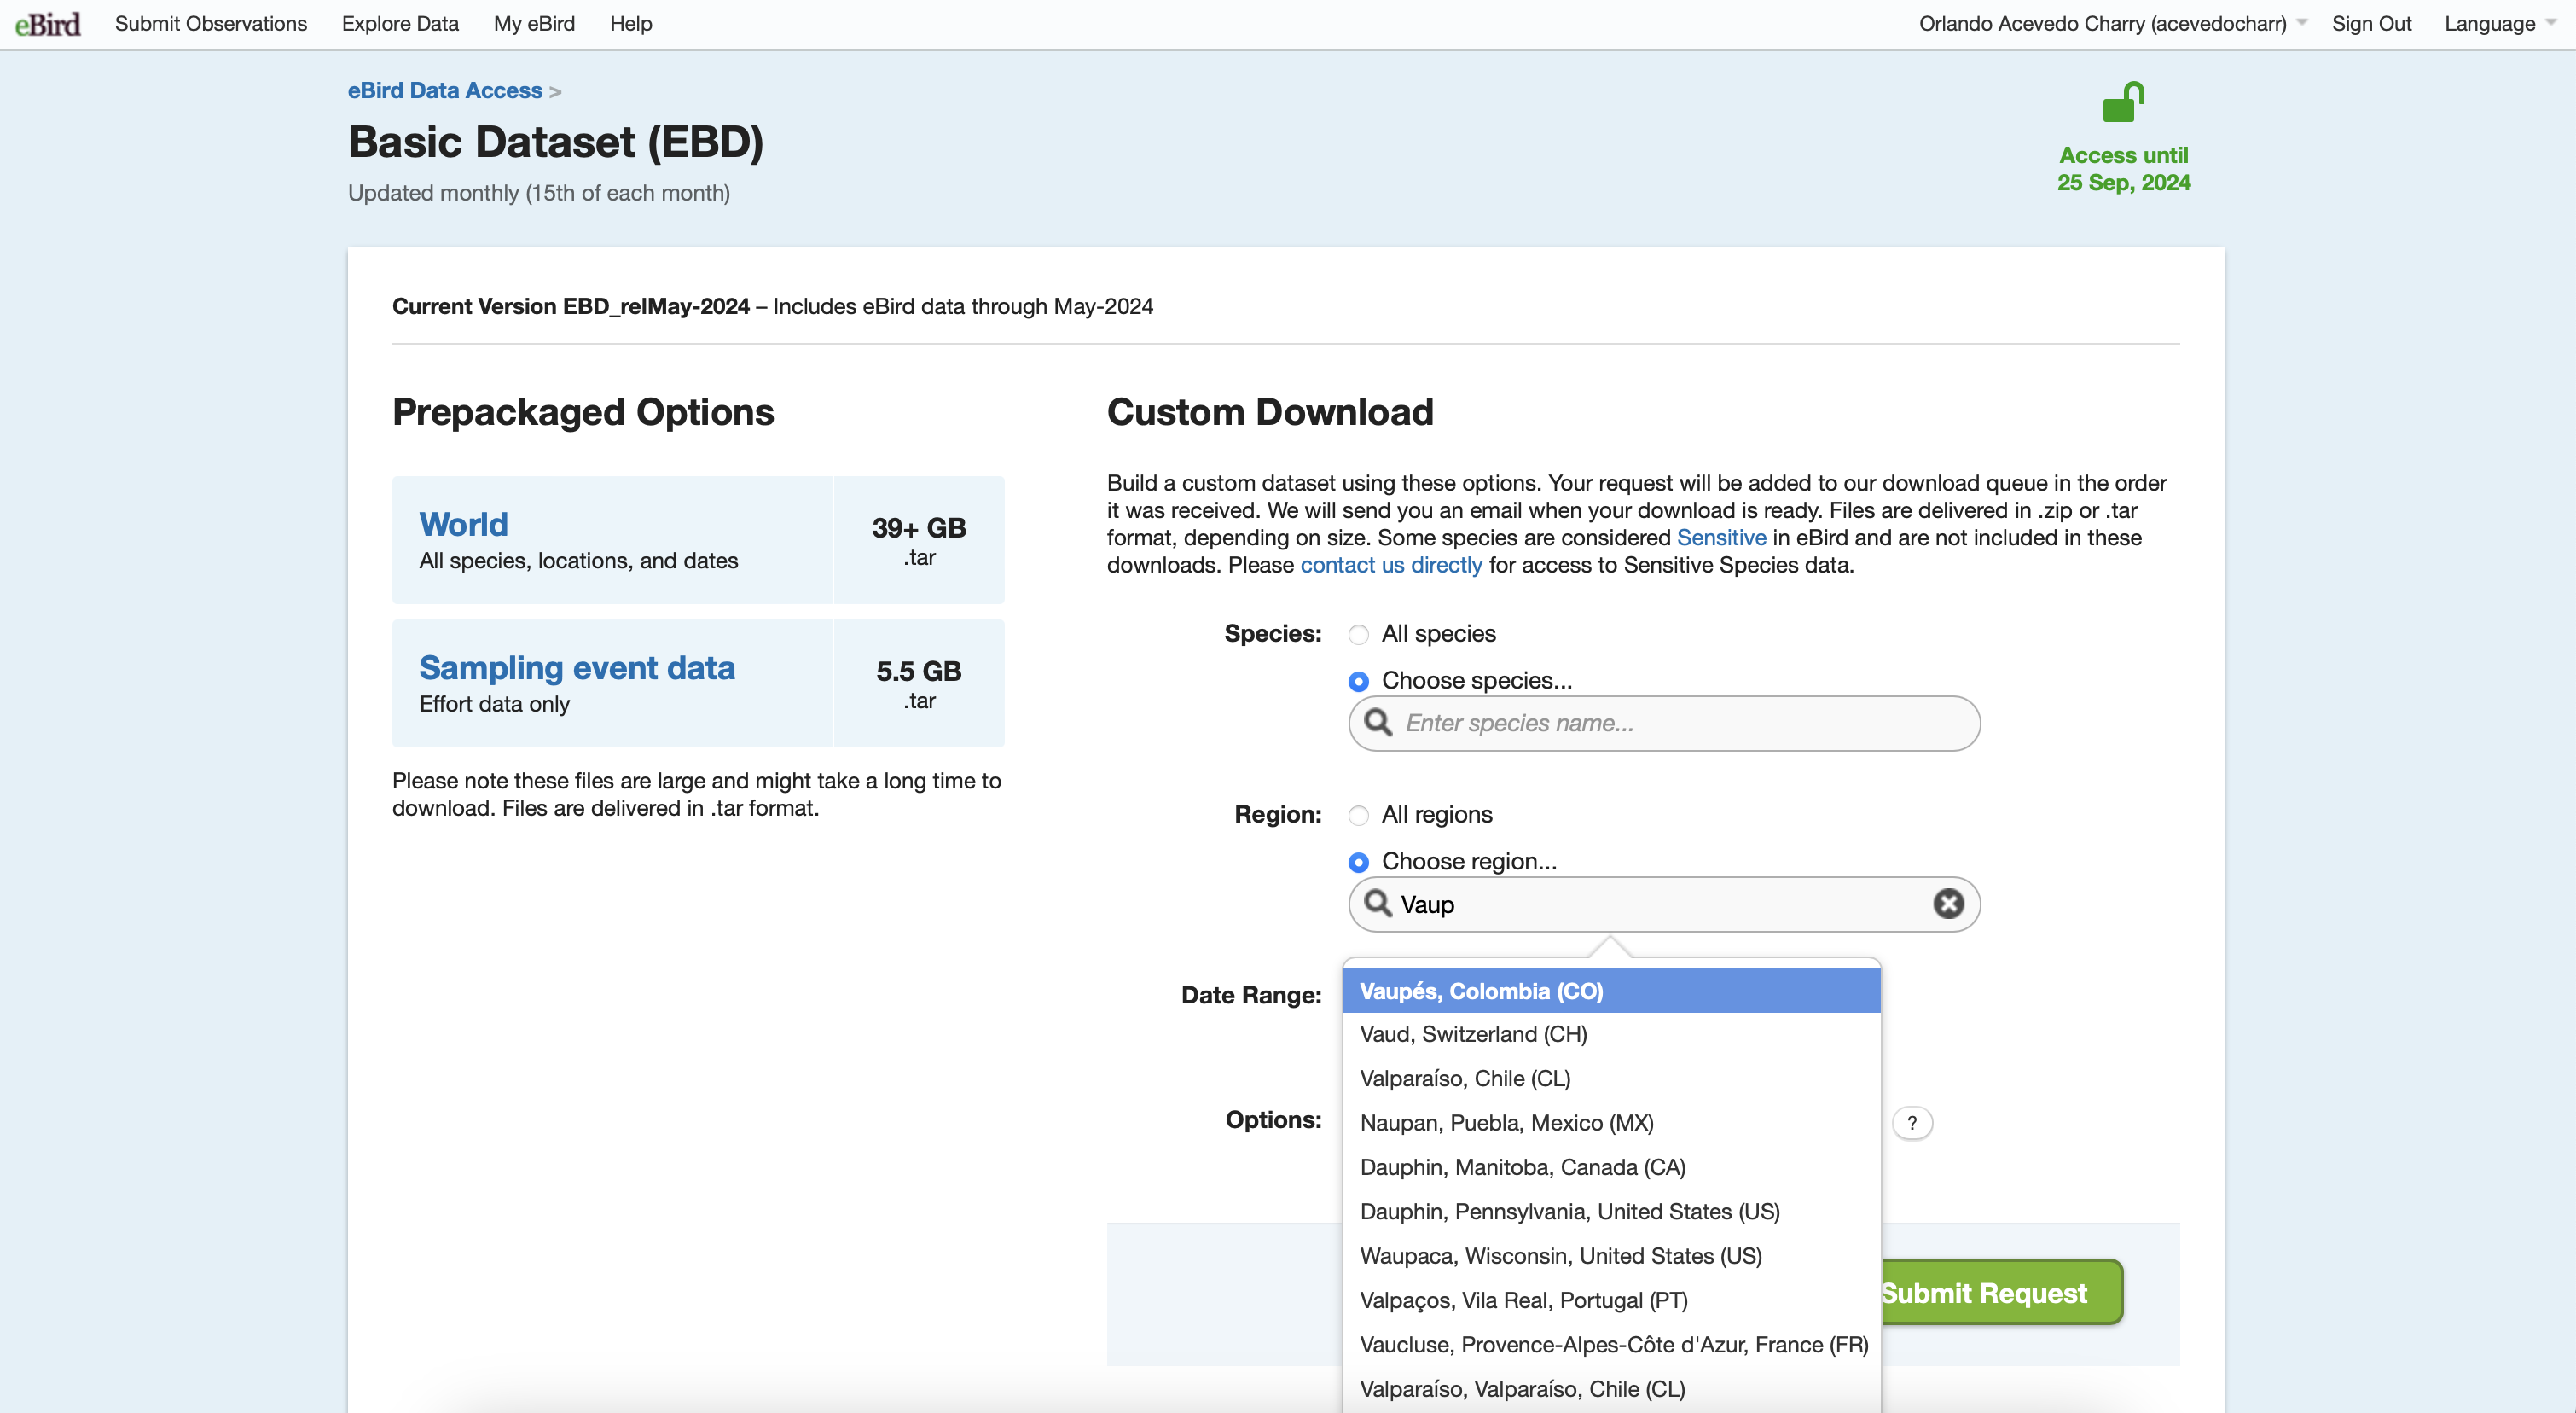
\includegraphics{screenshots/eBird4.png}
\caption{select region - seleccionar la región}
\end{figure}

When the download is ready, an email to your account will provide a link
to download the files. Move this folder to your working directory.

Cuando la descarga esté lista, un correo electrónico a su cuenta le va a
proveer un hipervínculo para descargar los archivos. Mueva esta carpeta
a su directorio de trabajo.

\begin{figure}
\centering
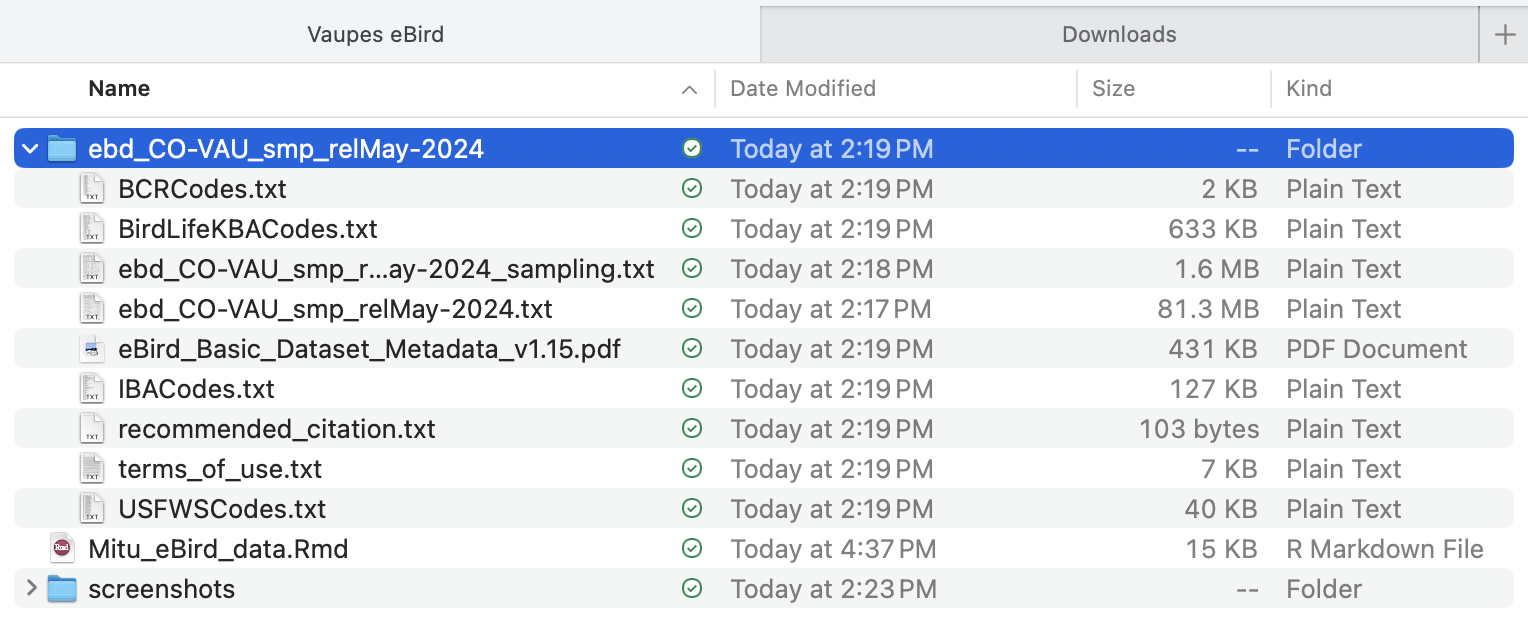
\includegraphics{screenshots/eBird5.png}
\caption{our working directory - nuestro directorio de trabajo}
\end{figure}

This folder has many files, the two files of our interest are
\texttt{ebd\_CO-VAU\_smp\_relMay-2024\_sampling.txt} (sampling event
data) and \texttt{ebd\_CO-VAU\_smp\_relMay-2024.txt} (event data).

Esta carpeta tiene varios archivos, de nuestro interés son los dos
archivos \texttt{ebd\_CO-VAU\_smp\_relMay-2024\_sampling.txt} (datos de
evento de muestreo) and \texttt{ebd\_CO-VAU\_smp\_relMay-2024.txt}
(datos de evento).

\hypertarget{ebird-data-exploration---explorando-los-datos-de-ebird}{%
\subsection{2. eBird data exploration - explorando los datos de
eBird}\label{ebird-data-exploration---explorando-los-datos-de-ebird}}

The downloaded data include all the Vaupes department, we can see the
entire department and use filters to compare this data.

Los datos descargados incluyen todo el Vaupés, posemos ver el
departamento entero y usar filtros para compara los datos.

\begin{Shaded}
\begin{Highlighting}[]
\NormalTok{f\_ebd }\OtherTok{\textless{}{-}} \StringTok{"temporal/ebd\_Mitu.txt"}                         \CommentTok{\#Data to be saved}
\NormalTok{f\_sed }\OtherTok{\textless{}{-}} \StringTok{"temporal/sed\_Mitu.txt"}                         \CommentTok{\#Sampling event to be saved}

\CommentTok{\#select the columns to extract (based on x$col\_idx$name)}
\NormalTok{colsE }\OtherTok{\textless{}{-}} \FunctionTok{c}\NormalTok{(}\StringTok{"observer\_id"}\NormalTok{, }\StringTok{"sampling\_event\_identifier"}\NormalTok{,}
           \StringTok{"group identifier"}\NormalTok{,}
           \StringTok{"common\_name"}\NormalTok{, }\StringTok{"scientific\_name"}\NormalTok{,}
           \StringTok{"observation\_count"}\NormalTok{,}
           \StringTok{"state\_code"}\NormalTok{, }\StringTok{"locality\_id"}\NormalTok{, }\StringTok{"latitude"}\NormalTok{, }\StringTok{"longitude"}\NormalTok{,}
           \StringTok{"protocol\_type"}\NormalTok{, }\StringTok{"all\_species\_reported"}\NormalTok{,}
           \StringTok{"observation\_date"}\NormalTok{,}
           \StringTok{"time\_observations\_started"}\NormalTok{,}
           \StringTok{"duration\_minutes"}\NormalTok{, }\StringTok{"effort\_distance\_km"}\NormalTok{,}
           \StringTok{"number\_observers"}\NormalTok{)}

\NormalTok{ebd\_filt}\OtherTok{\textless{}{-}}\FunctionTok{auk\_ebd}\NormalTok{(}\StringTok{"ebd\_CO{-}VAU\_smp\_relMay{-}2024/ebd\_CO{-}VAU\_smp\_relMay{-}2024.txt"}\NormalTok{,}
                  \AttributeTok{file\_sampling =} \StringTok{"ebd\_CO{-}VAU\_smp\_relMay{-}2024/ebd\_CO{-}VAU\_smp\_relMay{-}2024\_sampling.txt"}\NormalTok{) }\SpecialCharTok{\%\textgreater{}\%}
\CommentTok{\#  auk\_bbox(c({-}70.378, 0.835,{-}69.851, 1.325)) \%\textgreater{}\% \#W, S, E, N}
  \FunctionTok{auk\_filter}\NormalTok{(f\_ebd, f\_sed, }\AttributeTok{overwrite=}\NormalTok{T, }\AttributeTok{keep =}\NormalTok{ colsE)}
\end{Highlighting}
\end{Shaded}

\begin{verbatim}
## Warning in auk_filter.auk_ebd(., f_ebd, f_sed, overwrite = T, keep = colsE):
## Sampling event data file provided, but filters have not been set to only return
## complete checklists. Complete checklists are required for zero-filling. You may
## want to use auk_complete(), or manually filter out incomplete checklists.
\end{verbatim}

\begin{Shaded}
\begin{Highlighting}[]
\CommentTok{\#and with read\_ebd I apply another filter to do not repeate records from groups}
\NormalTok{sed\_only }\OtherTok{\textless{}{-}} \FunctionTok{read\_sampling}\NormalTok{(f\_sed)}
\NormalTok{ebd\_only }\OtherTok{\textless{}{-}} \FunctionTok{read\_ebd}\NormalTok{(f\_ebd)}
\end{Highlighting}
\end{Shaded}

This dataset include ``complete'' and ``incomplete'' lists. Our first
exploration could be regarding this categorical variable

Este conjunto de datos incluye listas ``completas'' e ``incompletas''.
Nuestra primera exploración puede ser con base a esta variable
categórica

\begin{Shaded}
\begin{Highlighting}[]
\NormalTok{ebd\_only }\SpecialCharTok{\%\textgreater{}\%}
  \FunctionTok{group\_by}\NormalTok{(all\_species\_reported) }\SpecialCharTok{\%\textgreater{}\%}
  \FunctionTok{summarise}\NormalTok{(}\AttributeTok{n\_records =} \FunctionTok{n}\NormalTok{())}
\end{Highlighting}
\end{Shaded}

\begin{verbatim}
## # A tibble: 2 x 2
##   all_species_reported n_records
##   <lgl>                    <int>
## 1 FALSE                     9167
## 2 TRUE                    113531
\end{verbatim}

Another exploration is the geographic extend of sampling effort (we can
use \texttt{sed\_only}). A simple map will be help to see where in the
department eBird has been used.

Otra exploración es la extensión geográfica del esfuerzo de muestreo
(podemos usar \texttt{sed\_only}). Un simple mapa nos ayudará a ver
donde eBird se ha usado en el departamento.

\begin{Shaded}
\begin{Highlighting}[]
\CommentTok{\#A global map to make figures }\AlertTok{\#\#\#}
\NormalTok{world1 }\OtherTok{\textless{}{-}}\NormalTok{ sf}\SpecialCharTok{::}\FunctionTok{st\_as\_sf}\NormalTok{(maps}\SpecialCharTok{::}\FunctionTok{map}\NormalTok{(}\AttributeTok{database =} \StringTok{\textquotesingle{}world\textquotesingle{}}\NormalTok{, }\AttributeTok{plot =} \ConstantTok{FALSE}\NormalTok{, }\AttributeTok{fill =} \ConstantTok{TRUE}\NormalTok{))}

\FunctionTok{ggplot}\NormalTok{()}\SpecialCharTok{+}
  \FunctionTok{geom\_sf}\NormalTok{(}\AttributeTok{data =}\NormalTok{ world1)}\SpecialCharTok{+}
  \FunctionTok{coord\_sf}\NormalTok{(}\AttributeTok{xlim =} \FunctionTok{c}\NormalTok{(}\SpecialCharTok{{-}}\FloatTok{71.477}\NormalTok{, }\SpecialCharTok{{-}}\FloatTok{69.353}\NormalTok{), }
           \AttributeTok{ylim =}  \FunctionTok{c}\NormalTok{(}\SpecialCharTok{{-}}\FloatTok{1.10711}\NormalTok{, }\FloatTok{1.35211}\NormalTok{)) }\SpecialCharTok{+}
  \FunctionTok{geom\_point}\NormalTok{(}\AttributeTok{data =}\NormalTok{ sed\_only, }
             \FunctionTok{aes}\NormalTok{(}\AttributeTok{x =}\NormalTok{ longitude, }\AttributeTok{y =}\NormalTok{ latitude), }
             \AttributeTok{size =} \FloatTok{0.5}\NormalTok{, }
             \AttributeTok{alpha =} \FloatTok{0.25}\NormalTok{)}\SpecialCharTok{+}
  \FunctionTok{labs}\NormalTok{(}\AttributeTok{title =} \StringTok{"eBird Sampling effort in Vaupés, Colombia"}\NormalTok{)}\SpecialCharTok{+}
  \FunctionTok{theme\_bw}\NormalTok{()}
\end{Highlighting}
\end{Shaded}

\includegraphics{Mitu_eBird_data_files/figure-latex/unnamed-chunk-4-1.pdf}

We can explore the data filtered to our study site, and assess different
aspects, such as the number of checklists per protocol, spatiotemporal
sampling effort.

Podemos explorar los datos filtrados en nuestro sitio de estudio y
evaluar diferentes aspectos, como el numero de listas por protocolo o
esfuerzo espacio temporal.

\hypertarget{protocol-type---tipo-de-protocolo}{%
\subsubsection{2.1 Protocol type - tipo de
protocolo}\label{protocol-type---tipo-de-protocolo}}

\begin{Shaded}
\begin{Highlighting}[]
\CommentTok{\#Explore some sampling effort information {-} Protocol type}

\FunctionTok{print}\NormalTok{(}\FunctionTok{table}\NormalTok{(ebd\_only}\SpecialCharTok{$}\NormalTok{protocol\_type)) }\CommentTok{\#to see the names and overall count}
\end{Highlighting}
\end{Shaded}

\begin{verbatim}
## 
##       Area    Banding Historical Incidental Stationary  Traveling 
##         29         93       8827       5054       4600     104095
\end{verbatim}

\begin{Shaded}
\begin{Highlighting}[]
\NormalTok{ebd\_only }\SpecialCharTok{\%\textgreater{}\%}
  \FunctionTok{group\_by}\NormalTok{(sampling\_event\_identifier, protocol\_type) }\SpecialCharTok{\%\textgreater{}\%} 
  \FunctionTok{summarise}\NormalTok{() }\SpecialCharTok{\%\textgreater{}\%} 
  \FunctionTok{ggplot}\NormalTok{(}\FunctionTok{aes}\NormalTok{(}\AttributeTok{x =} \FunctionTok{factor}\NormalTok{(protocol\_type, }
                        \AttributeTok{levels =} \FunctionTok{c}\NormalTok{(}\StringTok{"Traveling"}\NormalTok{,}
                                   \StringTok{"Stationary"}\NormalTok{,}
                                   \StringTok{"Incidental"}\NormalTok{,}
                                   \StringTok{"Historical"}\NormalTok{,}
                                   \StringTok{"Banding"}\NormalTok{,}\StringTok{"Area"}\NormalTok{))))}\SpecialCharTok{+}
    \FunctionTok{geom\_bar}\NormalTok{(}\AttributeTok{stat =} \StringTok{"count"}\NormalTok{)}\SpecialCharTok{+}
    \FunctionTok{stat\_count}\NormalTok{(}\AttributeTok{geom =} \StringTok{"text"}\NormalTok{, }\AttributeTok{colour =} \StringTok{"white"}\NormalTok{, }\AttributeTok{size =} \FloatTok{3.5}\NormalTok{,}
               \FunctionTok{aes}\NormalTok{(}\AttributeTok{label =} \FunctionTok{after\_stat}\NormalTok{(count)), }\AttributeTok{position=}\FunctionTok{position\_stack}\NormalTok{(}\AttributeTok{vjust=}\FloatTok{0.5}\NormalTok{))}\SpecialCharTok{+}
  \FunctionTok{labs}\NormalTok{(}\AttributeTok{title =} \StringTok{"Protocol {-} Protocolo"}\NormalTok{,}
       \AttributeTok{x =} \StringTok{""}\NormalTok{,}
       \AttributeTok{y =} \StringTok{"\# Checklists {-} listas"}\NormalTok{)}\SpecialCharTok{+}
  \FunctionTok{theme\_classic}\NormalTok{()}\SpecialCharTok{+}
  \FunctionTok{theme}\NormalTok{(}\AttributeTok{axis.text.x =} \FunctionTok{element\_text}\NormalTok{(}\AttributeTok{angle =} \DecValTok{65}\NormalTok{, }\AttributeTok{hjust =} \DecValTok{1}\NormalTok{, }\AttributeTok{vjust =} \DecValTok{1}\NormalTok{))}
\end{Highlighting}
\end{Shaded}

\begin{verbatim}
## `summarise()` has grouped output by 'sampling_event_identifier'. You can
## override using the `.groups` argument.
\end{verbatim}

\includegraphics{Mitu_eBird_data_files/figure-latex/unnamed-chunk-5-1.pdf}

\begin{Shaded}
\begin{Highlighting}[]
\CommentTok{\#which checklist includes "Banding" or "Area" protocols?}

\NormalTok{ebd\_only }\SpecialCharTok{|\textgreater{}}
  \FunctionTok{filter}\NormalTok{(protocol\_type }\SpecialCharTok{\%in\%} \FunctionTok{c}\NormalTok{(}\StringTok{"Banding"}\NormalTok{, }\StringTok{"Area"}\NormalTok{)) }\SpecialCharTok{|\textgreater{}}
  \FunctionTok{select}\NormalTok{(sampling\_event\_identifier) }\SpecialCharTok{|\textgreater{}}
  \FunctionTok{unique}\NormalTok{()}
\end{Highlighting}
\end{Shaded}

\begin{verbatim}
## # A tibble: 2 x 1
##   sampling_event_identifier
##   <chr>                    
## 1 S36819056                
## 2 S55879500
\end{verbatim}

We can see that two checklists include ``Banding'' or ``Area''
protocols. ``Banding'' records came from the checklists
\href{https://ebird.org/checklist/S36819056}{S36819056}. This list
occurred during mist netting activity (Agripino González with the Sinchi
Institute), but for sure the list do not report only the captured birds
for banding (best recommendation). When working with mist nets, we
should submit two separated lists: one with all the birds heard or seen
(but not captured) under ``Traveling'' or ``Stationary'', and one ONLY
with the captured birds. On the other hand, records by ``Area''
checklist came from
\href{https://ebird.org/checklist/S55879500}{S55879500}, by a ``group''
account submission. Group accounts should not report the list primarily,
because we do not have a person to contact. This protocol is very
exhaustive for rigorous surveys, thus it might be a ``Traveling'' list.

Podemos ver que hay dos listas que incluyen ``Anillamiento'' o
``Busqueda intensa por área''. Los registros de la lista de
``Anillamiento'' son de
\href{https://ebird.org/checklist/S36819056}{S36819056}. Esta lista
ocurrió durante actividad de redes de niebla (Agripino González con el
Instituto Sinchi),pero la lista seguramente no está reportando solo las
aves caputradas para anillar (mejor recomendación).Cuando se trabaje con
redes de niebla, uno deberia someter dos listas separadas: una para las
aves vistas y escuchadas (pero no capturadas) siguiendo protocolos de
``desplazamiento'' o ``estacionario'', y otra SOLO con las aves
capturadas. Por otro lado, los registros de la lista de ``Busqueda
intensa por área'' vienen de
\href{https://ebird.org/checklist/S55879500}{S55879500}, sometida por
una cuenta grupal. Las cuentas grupales no deben reportar las listas,
pues no tenemos una persona real de contacto. Este protocolo es muy
exahustivo para muestreos rigurosos y repetitivos, entonces tal vez
debería responder mas a ``desplazamiento''.

We will focus in ``best practices'' records from ``Traveling'' and
``Stationary'' protocols. We can also explore the effort (duration,
distance, observers, hour of sampling).

First, we have to do some adjustment to the data:

Vamos a enfocarnos en los registros con ``mejores prácticas'' dentro de
los protocolos ``desplazamiento'' y ``estacionario''. Podemos tambien
explorar el esfuerzo (duracion, distancia, \# observadores, horas de
muestreo).

Primero debemos hacer algunos ajustes a los datos:

\begin{Shaded}
\begin{Highlighting}[]
\CommentTok{\# Function to convert time observation to hours since midnight}
\NormalTok{time\_to\_decimal }\OtherTok{\textless{}{-}} \ControlFlowTok{function}\NormalTok{(x) \{}
\NormalTok{  x }\OtherTok{\textless{}{-}} \FunctionTok{hms}\NormalTok{(x, }\AttributeTok{quiet =} \ConstantTok{TRUE}\NormalTok{)}
  \FunctionTok{hour}\NormalTok{(x) }\SpecialCharTok{+} \FunctionTok{minute}\NormalTok{(x) }\SpecialCharTok{/} \DecValTok{60} \SpecialCharTok{+} \FunctionTok{second}\NormalTok{(x) }\SpecialCharTok{/} \DecValTok{3600}
\NormalTok{\}}

\CommentTok{\# clean up variables}
\NormalTok{ebd\_count }\OtherTok{\textless{}{-}}\NormalTok{ ebd\_only }\SpecialCharTok{\%\textgreater{}\%}
  \FunctionTok{mutate}\NormalTok{(}
    \CommentTok{\# We don\textquotesingle{}t have here count in X to convert to NA}
    \AttributeTok{observation\_count =} \FunctionTok{as.integer}\NormalTok{(observation\_count),}
    \CommentTok{\# effort\_distance\_km to 0 for non{-}travelling counts}
    \AttributeTok{effort\_distance\_km =} \FunctionTok{if\_else}\NormalTok{(protocol\_type }\SpecialCharTok{==} \StringTok{"Stationary"}\NormalTok{,}
                                 \DecValTok{0}\NormalTok{, effort\_distance\_km),}
    \CommentTok{\#effort\_distance\_km change to integer no decimals}
    \AttributeTok{effort\_distance\_kmI =} \FunctionTok{round}\NormalTok{(effort\_distance\_km, }\AttributeTok{digits =} \DecValTok{0}\NormalTok{),}
    \CommentTok{\# convert time to decimal hours since midnight}
    \AttributeTok{time\_observations\_started =} \FunctionTok{time\_to\_decimal}\NormalTok{(time\_observations\_started),}
    \CommentTok{\# split date into year, month, week, and day of year}
    \AttributeTok{year =} \FunctionTok{year}\NormalTok{(observation\_date),}
    \AttributeTok{month =} \FunctionTok{month}\NormalTok{(observation\_date),}
    \AttributeTok{week =} \FunctionTok{week}\NormalTok{(observation\_date),}
    \AttributeTok{day\_of\_year =} \FunctionTok{yday}\NormalTok{(observation\_date))}
\end{Highlighting}
\end{Shaded}

\begin{verbatim}
## Warning: There was 1 warning in `mutate()`.
## i In argument: `observation_count = as.integer(observation_count)`.
## Caused by warning:
## ! NAs introduced by coercion
\end{verbatim}

\begin{Shaded}
\begin{Highlighting}[]
\NormalTok{ebd\_count }\OtherTok{\textless{}{-}}\NormalTok{ ebd\_count }\SpecialCharTok{|\textgreater{}}
  \FunctionTok{group\_by}\NormalTok{(sampling\_event\_identifier) }\SpecialCharTok{|\textgreater{}}
  \FunctionTok{summarise}\NormalTok{(}\AttributeTok{Total\_ind =} \FunctionTok{sum}\NormalTok{(observation\_count, }\AttributeTok{na.rm =}\NormalTok{ T)) }\SpecialCharTok{|\textgreater{}}
  \FunctionTok{left\_join}\NormalTok{(ebd\_count)}
\end{Highlighting}
\end{Shaded}

\begin{verbatim}
## Joining with `by = join_by(sampling_event_identifier)`
\end{verbatim}

With this, we can assign each observation to different groups.

Con esto, podemos asignar cada observación a diferentes grupos.

\hypertarget{assigning-each-record-to-detail-of-sampling---asignando-cada-registro-en-referencia-al-detalle-de-muestreo}{%
\subsection{3. Assigning each record to detail of sampling - asignando
cada registro en referencia al detalle de
muestreo}\label{assigning-each-record-to-detail-of-sampling---asignando-cada-registro-en-referencia-al-detalle-de-muestreo}}

Podemos plantear diferentes niveles de resolución de esfuerzo, el primer
paso para saber cómo analizar estos datos:

\begin{enumerate}
\def\labelenumi{\arabic{enumi}.}
\tightlist
\item
  ``Ultrafine'': una resolución super fina incluye solo listas
  compeltas, estacionarias, por un solo observador, entre 20-30 minutos,
  reportando al menos 15 individuos, e incluyendo estimación de
  abundancia para cada especie. A esta o la siguiente (Fine) deberíamos
  apuntar a llegar!
\end{enumerate}

\begin{Shaded}
\begin{Highlighting}[]
\NormalTok{Ultrafine }\OtherTok{\textless{}{-}}\NormalTok{ ebd\_count }\SpecialCharTok{|\textgreater{}}
  \FunctionTok{filter}\NormalTok{(all\_species\_reported }\SpecialCharTok{==} \StringTok{"TRUE"}\NormalTok{,}
\NormalTok{         protocol\_type }\SpecialCharTok{==} \StringTok{"Stationary"}\NormalTok{,}
\NormalTok{         number\_observers }\SpecialCharTok{==} \DecValTok{1}\NormalTok{,}
\NormalTok{         duration\_minutes }\SpecialCharTok{\%in\%} \FunctionTok{c}\NormalTok{(}\DecValTok{20}\SpecialCharTok{:}\DecValTok{30}\NormalTok{),}
\NormalTok{         Total\_ind }\SpecialCharTok{\textgreater{}=} \DecValTok{15}\NormalTok{) }\SpecialCharTok{|\textgreater{}}
  \FunctionTok{drop\_na}\NormalTok{(observation\_count) }\SpecialCharTok{|\textgreater{}}
  \FunctionTok{mutate}\NormalTok{(}\AttributeTok{Grupo =} \StringTok{"Ultrafine"}\NormalTok{)}
\end{Highlighting}
\end{Shaded}

\begin{enumerate}
\def\labelenumi{\arabic{enumi}.}
\setcounter{enumi}{1}
\tightlist
\item
  ``Fine'': resolución fina (interesante para encontrar bosques de
  arenas blancas). Solo listas completas, de ``traveling'' o
  ``stationary'' con un esfuerzo ≥1 km o entre 5 minutos a 1 hora, hasta
  10 observadores, e incluyendo estimación de abundancia para cada
  especie.
\end{enumerate}

\begin{Shaded}
\begin{Highlighting}[]
\NormalTok{Fine }\OtherTok{\textless{}{-}}\NormalTok{ ebd\_count }\SpecialCharTok{|\textgreater{}}
  \FunctionTok{filter}\NormalTok{(all\_species\_reported }\SpecialCharTok{==} \StringTok{"TRUE"}\NormalTok{,}
\NormalTok{         protocol\_type }\SpecialCharTok{\%in\%} \FunctionTok{c}\NormalTok{(}\StringTok{"Stationary"}\NormalTok{, }\StringTok{"Traveling"}\NormalTok{),}
\NormalTok{         duration\_minutes }\SpecialCharTok{\%in\%} \FunctionTok{c}\NormalTok{(}\DecValTok{5}\SpecialCharTok{:}\DecValTok{60}\NormalTok{),}
\NormalTok{         effort\_distance\_kmI }\SpecialCharTok{\%in\%} \FunctionTok{c}\NormalTok{(}\DecValTok{0}\SpecialCharTok{:}\DecValTok{1}\NormalTok{),}
\NormalTok{         number\_observers }\SpecialCharTok{\%in\%} \FunctionTok{c}\NormalTok{(}\DecValTok{1}\SpecialCharTok{:}\DecValTok{10}\NormalTok{)) }\SpecialCharTok{|\textgreater{}}
  \FunctionTok{drop\_na}\NormalTok{(observation\_count)}\SpecialCharTok{|\textgreater{}}
  \FunctionTok{mutate}\NormalTok{(}\AttributeTok{Grupo =} \StringTok{"Fine"}\NormalTok{)}
\end{Highlighting}
\end{Shaded}

\begin{enumerate}
\def\labelenumi{\arabic{enumi}.}
\setcounter{enumi}{2}
\tightlist
\item
  ``Coarse'': resolución gruesa, pero es la estandarizada que se usa a
  nivel mundial en escalas macroecológicas. Incluye listas completas de
  ``traveling'' o ``stationary'' con un esfuerzo ≥5 km o entre 5 minutos
  a 5 horas (300 minutos) de muestreo, hasta 10 observadores, y que
  incluyan estimación de abundancia de las especies reportadas.
\end{enumerate}

\begin{Shaded}
\begin{Highlighting}[]
\NormalTok{Coarse }\OtherTok{\textless{}{-}}\NormalTok{ ebd\_count }\SpecialCharTok{|\textgreater{}}
  \FunctionTok{filter}\NormalTok{(all\_species\_reported }\SpecialCharTok{==} \StringTok{"TRUE"}\NormalTok{,}
\NormalTok{         protocol\_type }\SpecialCharTok{\%in\%} \FunctionTok{c}\NormalTok{(}\StringTok{"Stationary"}\NormalTok{, }\StringTok{"Traveling"}\NormalTok{),}
\NormalTok{         duration\_minutes }\SpecialCharTok{\%in\%} \FunctionTok{c}\NormalTok{(}\DecValTok{5}\SpecialCharTok{:}\DecValTok{300}\NormalTok{),}
\NormalTok{         effort\_distance\_kmI }\SpecialCharTok{\%in\%} \FunctionTok{c}\NormalTok{(}\DecValTok{0}\SpecialCharTok{:}\DecValTok{5}\NormalTok{), }
\NormalTok{         number\_observers }\SpecialCharTok{\%in\%} \FunctionTok{c}\NormalTok{(}\DecValTok{1}\SpecialCharTok{:}\DecValTok{10}\NormalTok{)) }\SpecialCharTok{|\textgreater{}}
  \FunctionTok{drop\_na}\NormalTok{(observation\_count) }\SpecialCharTok{|\textgreater{}}
  \FunctionTok{mutate}\NormalTok{(}\AttributeTok{Grupo =} \StringTok{"Coarse"}\NormalTok{)}
\end{Highlighting}
\end{Shaded}

\begin{enumerate}
\def\labelenumi{\arabic{enumi}.}
\setcounter{enumi}{3}
\tightlist
\item
  ``Room for improvement'': incluir listas completas de cualquier otro
  protocolo, por mas de 5 horas o por mas de 5 km, e incluyendo mas de
  10 observadores.
\end{enumerate}

\begin{Shaded}
\begin{Highlighting}[]
\NormalTok{ToImprove }\OtherTok{\textless{}{-}}\NormalTok{ ebd\_count }\SpecialCharTok{|\textgreater{}}
  \FunctionTok{filter}\NormalTok{(all\_species\_reported }\SpecialCharTok{==} \StringTok{"TRUE"}\NormalTok{,}
\NormalTok{         protocol\_type }\SpecialCharTok{\%in\%} \FunctionTok{c}\NormalTok{(}\StringTok{"Area"}\NormalTok{,}
                              \StringTok{"Banding"}\NormalTok{,}
                              \StringTok{"Historical"}\NormalTok{,}
                              \StringTok{"Incidental"}\NormalTok{) }\SpecialCharTok{|}
\NormalTok{         duration\_minutes }\SpecialCharTok{\%in\%} \FunctionTok{c}\NormalTok{(}\DecValTok{1}\SpecialCharTok{:}\DecValTok{4}\NormalTok{,}\DecValTok{300}\SpecialCharTok{:}\DecValTok{1440}\NormalTok{) }\SpecialCharTok{|} 
\NormalTok{         effort\_distance\_kmI }\SpecialCharTok{\textgreater{}} \DecValTok{5} \SpecialCharTok{|}
\NormalTok{         number\_observers }\SpecialCharTok{\textgreater{}} \DecValTok{10} \SpecialCharTok{|}
         \FunctionTok{is.na}\NormalTok{(observation\_count)) }\SpecialCharTok{|\textgreater{}}
  \FunctionTok{mutate}\NormalTok{(}\AttributeTok{Grupo =} \StringTok{"ToImprove"}\NormalTok{)}
\end{Highlighting}
\end{Shaded}

\begin{enumerate}
\def\labelenumi{\arabic{enumi}.}
\setcounter{enumi}{4}
\tightlist
\item
  ``Incomplete'' son las listas correctamente identificadas como
  incompletas, las cuales al momento de analizar, por lo general, se
  filtran, pues no hay certeza de algunos aspectos del muestreo.
\end{enumerate}

\begin{Shaded}
\begin{Highlighting}[]
\NormalTok{Incomplete }\OtherTok{\textless{}{-}}\NormalTok{ ebd\_count }\SpecialCharTok{|\textgreater{}}
  \FunctionTok{filter}\NormalTok{(all\_species\_reported }\SpecialCharTok{==} \StringTok{"FALSE"}\NormalTok{) }\SpecialCharTok{|\textgreater{}}
  \FunctionTok{mutate}\NormalTok{(}\AttributeTok{Grupo =} \StringTok{"Incomplete"}\NormalTok{)}
\end{Highlighting}
\end{Shaded}

Combinar ahora los grupos

\begin{Shaded}
\begin{Highlighting}[]
\NormalTok{Grupos }\OtherTok{\textless{}{-}} \FunctionTok{rbind}\NormalTok{(Ultrafine, Fine, Coarse, ToImprove, Incomplete)}

\NormalTok{ebd\_eff }\OtherTok{\textless{}{-}}\NormalTok{ ebd\_count }\SpecialCharTok{|\textgreater{}}
  \FunctionTok{left\_join}\NormalTok{(Grupos) }\CommentTok{\#some checklists classify in different groups}
\end{Highlighting}
\end{Shaded}

\begin{verbatim}
## Joining with `by = join_by(sampling_event_identifier, Total_ind, checklist_id,
## common_name, scientific_name, observation_count, state_code, locality_id,
## latitude, longitude, observation_date, time_observations_started, observer_id,
## protocol_type, duration_minutes, effort_distance_km, number_observers,
## all_species_reported, group_identifier, effort_distance_kmI, year, month, week,
## day_of_year)`
\end{verbatim}

\begin{Shaded}
\begin{Highlighting}[]
\FunctionTok{table}\NormalTok{(ebd\_eff}\SpecialCharTok{$}\NormalTok{Grupo)}
\end{Highlighting}
\end{Shaded}

\begin{verbatim}
## 
##     Coarse       Fine Incomplete  ToImprove  Ultrafine 
##      41971       7009       9167      73764        102
\end{verbatim}

\begin{Shaded}
\begin{Highlighting}[]
\FunctionTok{nrow}\NormalTok{(ebd\_eff)}\SpecialCharTok{{-}}\FunctionTok{sum}\NormalTok{(}\DecValTok{41276}\NormalTok{,}\DecValTok{6941}\NormalTok{,}\DecValTok{8800}\NormalTok{,}\DecValTok{72677}\NormalTok{,}\DecValTok{102}\NormalTok{)}
\end{Highlighting}
\end{Shaded}

\begin{verbatim}
## [1] 2217
\end{verbatim}

\hypertarget{distribution-of-the-records---distribuciuxf3n-de-los-registros}{%
\subsection{4. Distribution of the records - distribución de los
registros}\label{distribution-of-the-records---distribuciuxf3n-de-los-registros}}

Hacer un ``Sankey plot'', como el flujo de numero de registros entre los
diferentes niveles de filtrar los datos, resultando a las cinco
categorías utilizadas.

\begin{Shaded}
\begin{Highlighting}[]
\NormalTok{ebd\_eff }\OtherTok{\textless{}{-}}\NormalTok{ ebd\_eff }\SpecialCharTok{|\textgreater{}}
  \FunctionTok{mutate}\NormalTok{(}\AttributeTok{All =} \StringTok{"eBird Vaupés (CO) {-} 122,796"}\NormalTok{,}
         \AttributeTok{Lists =} \FunctionTok{case\_when}\NormalTok{(all\_species\_reported }\SpecialCharTok{==} \ConstantTok{FALSE} \SpecialCharTok{\textasciitilde{}} \StringTok{"b. Incomplete {-} 6.8\%"}\NormalTok{,}
\NormalTok{                              all\_species\_reported }\SpecialCharTok{==} \ConstantTok{TRUE} \SpecialCharTok{\textasciitilde{}}\StringTok{"a. Complete {-} 93.2\%"}\NormalTok{),}
         \AttributeTok{Protocol =} \FunctionTok{case\_when}\NormalTok{(protocol\_type }\SpecialCharTok{==} \StringTok{"Area"} \SpecialCharTok{\textasciitilde{}} \StringTok{"e. Area and Banding {-} \textless{}1\%"}\NormalTok{,}
\NormalTok{                              protocol\_type }\SpecialCharTok{==} \StringTok{"Banding"} \SpecialCharTok{\textasciitilde{}} \StringTok{"e. Area and Banding {-} \textless{}1\%"}\NormalTok{,}
\NormalTok{                              protocol\_type }\SpecialCharTok{==} \StringTok{"Historical"} \SpecialCharTok{\textasciitilde{}} \StringTok{"b. Historical {-} 6.4\%"}\NormalTok{,}
\NormalTok{                              protocol\_type }\SpecialCharTok{==} \StringTok{"Incidental"} \SpecialCharTok{\textasciitilde{}} \StringTok{"d. Incidental {-} 3.9\%"}\NormalTok{,}
\NormalTok{                              protocol\_type }\SpecialCharTok{==} \StringTok{"Stationary"} \SpecialCharTok{\textasciitilde{}} \StringTok{"c. Stationary {-} 4.8\%"}\NormalTok{,}
\NormalTok{                              protocol\_type }\SpecialCharTok{==} \StringTok{"Traveling"} \SpecialCharTok{\textasciitilde{}} \StringTok{"a. Traveling {-} 84.8\%"}\NormalTok{),}
         \AttributeTok{Duration =} \FunctionTok{case\_when}\NormalTok{(duration\_minutes }\SpecialCharTok{\%in\%} \FunctionTok{c}\NormalTok{(}\DecValTok{1}\SpecialCharTok{:}\DecValTok{5}\NormalTok{) }\SpecialCharTok{\textasciitilde{}} \StringTok{"a. 1{-}5 minutes {-} \textless{}1\%"}\NormalTok{,}
\NormalTok{                              duration\_minutes }\SpecialCharTok{\%in\%} \FunctionTok{c}\NormalTok{(}\DecValTok{5}\SpecialCharTok{:}\DecValTok{20}\NormalTok{) }\SpecialCharTok{\textasciitilde{}} \StringTok{"b. 5{-}20 minutes {-} 3.3\%"}\NormalTok{,}
\NormalTok{                              duration\_minutes }\SpecialCharTok{\%in\%} \FunctionTok{c}\NormalTok{(}\DecValTok{20}\SpecialCharTok{:}\DecValTok{30}\NormalTok{) }\SpecialCharTok{\textasciitilde{}} \StringTok{"c. 20{-}30 minutes {-} 2.3\%"}\NormalTok{,}
\NormalTok{                              duration\_minutes }\SpecialCharTok{\%in\%} \FunctionTok{c}\NormalTok{(}\DecValTok{30}\SpecialCharTok{:}\DecValTok{60}\NormalTok{) }\SpecialCharTok{\textasciitilde{}} \StringTok{"d. 0.5{-}1 hour {-} 6.6\%"}\NormalTok{,}
\NormalTok{                              duration\_minutes }\SpecialCharTok{\%in\%} \FunctionTok{c}\NormalTok{(}\DecValTok{60}\SpecialCharTok{:}\DecValTok{300}\NormalTok{) }\SpecialCharTok{\textasciitilde{}} \StringTok{"e. 1{-}5 hours {-} 37.0\%"}\NormalTok{,}
\NormalTok{                              duration\_minutes }\SpecialCharTok{\textgreater{}} \DecValTok{300} \SpecialCharTok{\textasciitilde{}} \StringTok{"f. \textgreater{}5 hours {-} 41.5\%"}\NormalTok{,}
                              \FunctionTok{is.na}\NormalTok{(duration\_minutes) }\SpecialCharTok{\textasciitilde{}} \StringTok{"NA {-} 8.5"}\NormalTok{),}
         \AttributeTok{Distance =} \FunctionTok{case\_when}\NormalTok{(effort\_distance\_kmI }\SpecialCharTok{\%in\%} \FunctionTok{c}\NormalTok{(}\DecValTok{0}\SpecialCharTok{:}\DecValTok{1}\NormalTok{) }\SpecialCharTok{\textasciitilde{}} \StringTok{"a. \textless{} 1 km {-} 18.8\%"}\NormalTok{,}
\NormalTok{                              effort\_distance\_kmI }\SpecialCharTok{\%in\%} \FunctionTok{c}\NormalTok{(}\DecValTok{1}\SpecialCharTok{:}\DecValTok{2}\NormalTok{) }\SpecialCharTok{\textasciitilde{}} \StringTok{"b. 1{-}2 km {-} 11.1\%"}\NormalTok{,}
\NormalTok{                              effort\_distance\_kmI }\SpecialCharTok{\%in\%} \FunctionTok{c}\NormalTok{(}\DecValTok{2}\SpecialCharTok{:}\DecValTok{5}\NormalTok{) }\SpecialCharTok{\textasciitilde{}} \StringTok{"c. 2{-}5 km {-} 28.1\%"}\NormalTok{,}
\NormalTok{                              effort\_distance\_kmI }\SpecialCharTok{\textgreater{}} \DecValTok{5} \SpecialCharTok{\textasciitilde{}} \StringTok{"d. \textgreater{}5 km {-} 32.3\%"}\NormalTok{,}
                              \FunctionTok{is.na}\NormalTok{(effort\_distance\_kmI) }\SpecialCharTok{\textasciitilde{}} \StringTok{"NA {-} 9.6\%"}\NormalTok{),}
         \AttributeTok{Observers =} \FunctionTok{case\_when}\NormalTok{(number\_observers }\SpecialCharTok{\%in\%} \FunctionTok{c}\NormalTok{(}\DecValTok{1}\NormalTok{) }\SpecialCharTok{\textasciitilde{}} \StringTok{"a. 1 eBirder {-} 12.6\%"}\NormalTok{,}
\NormalTok{                               number\_observers }\SpecialCharTok{\%in\%} \FunctionTok{c}\NormalTok{(}\DecValTok{2}\SpecialCharTok{:}\DecValTok{5}\NormalTok{) }\SpecialCharTok{\textasciitilde{}} \StringTok{"b. 2{-}5 eBirders {-} 55.4\%"}\NormalTok{,}
\NormalTok{                               number\_observers }\SpecialCharTok{\%in\%} \FunctionTok{c}\NormalTok{(}\DecValTok{5}\SpecialCharTok{:}\DecValTok{10}\NormalTok{) }\SpecialCharTok{\textasciitilde{}} \StringTok{"c. 5{-}10 eBirders {-} 22.1\%"}\NormalTok{,}
\NormalTok{                              number\_observers }\SpecialCharTok{\%in\%} \FunctionTok{c}\NormalTok{(}\DecValTok{10}\SpecialCharTok{:}\DecValTok{20}\NormalTok{) }\SpecialCharTok{\textasciitilde{}} \StringTok{"d. 10{-}20 eBirders {-} 5.6\%"}\NormalTok{,}
\NormalTok{                              number\_observers }\SpecialCharTok{\textgreater{}}\DecValTok{20} \SpecialCharTok{\textasciitilde{}} \StringTok{"e. \textgreater{}20 eBirders {-} \textless{}1\%"}\NormalTok{,}
                              \FunctionTok{is.na}\NormalTok{(number\_observers) }\SpecialCharTok{\textasciitilde{}} \StringTok{"NA {-} 4.3\%"}\NormalTok{),}
         \AttributeTok{Category =} \FunctionTok{case\_when}\NormalTok{(Grupo }\SpecialCharTok{==} \StringTok{"Ultrafine"} \SpecialCharTok{\textasciitilde{}} \StringTok{"a. Ultrafine {-} \textless{}1\%"}\NormalTok{,}
\NormalTok{                              Grupo }\SpecialCharTok{==} \StringTok{"Fine"} \SpecialCharTok{\textasciitilde{}} \StringTok{"b. Fine {-} 5.3\%"}\NormalTok{,}
\NormalTok{                              Grupo }\SpecialCharTok{==} \StringTok{"Coarse"} \SpecialCharTok{\textasciitilde{}} \StringTok{"c. Coarse {-} 31.8\%"}\NormalTok{,}
\NormalTok{                              Grupo }\SpecialCharTok{==} \StringTok{"ToImprove"} \SpecialCharTok{\textasciitilde{}} \StringTok{"d. Room for improvement {-} 56.0\%"}\NormalTok{,}
\NormalTok{                              Grupo }\SpecialCharTok{==} \StringTok{"Incomplete"} \SpecialCharTok{\textasciitilde{}} \StringTok{"e. Correctly removed {-} 6.7\%"}\NormalTok{,}
                              \FunctionTok{is.na}\NormalTok{(Grupo) }\SpecialCharTok{\textasciitilde{}} \StringTok{"Not Aplicable"}\NormalTok{))}

\NormalTok{dfVA\_CO }\OtherTok{\textless{}{-}}\NormalTok{ ebd\_eff }\SpecialCharTok{|\textgreater{}}
  \FunctionTok{make\_long}\NormalTok{(All, Lists, Protocol, Duration, Distance, Observers, Category)}

\FunctionTok{ggplot}\NormalTok{(dfVA\_CO, }\FunctionTok{aes}\NormalTok{(}\AttributeTok{x =}\NormalTok{ x, }\AttributeTok{next\_x =}\NormalTok{ next\_x, }\AttributeTok{node =}\NormalTok{ node, }\AttributeTok{next\_node =}\NormalTok{ next\_node, }\AttributeTok{fill =} \FunctionTok{factor}\NormalTok{(node), }\AttributeTok{label =}\NormalTok{ node)) }\SpecialCharTok{+}
  \FunctionTok{geom\_sankey}\NormalTok{(}\AttributeTok{flow.alpha =}\NormalTok{ .}\DecValTok{6}\NormalTok{,}
              \AttributeTok{node.color =} \StringTok{"gray30"}\NormalTok{) }\SpecialCharTok{+}
  \FunctionTok{geom\_sankey\_label}\NormalTok{(}\AttributeTok{size =} \FloatTok{2.5}\NormalTok{, }\AttributeTok{color =} \StringTok{"white"}\NormalTok{, }\AttributeTok{fill =} \StringTok{"gray40"}\NormalTok{) }\SpecialCharTok{+}
  \FunctionTok{scale\_fill\_viridis\_d}\NormalTok{(}\AttributeTok{drop =} \ConstantTok{FALSE}\NormalTok{) }\SpecialCharTok{+}
  \FunctionTok{theme\_sankey}\NormalTok{(}\AttributeTok{base\_size =} \DecValTok{18}\NormalTok{) }\SpecialCharTok{+}
  \FunctionTok{labs}\NormalTok{(}\AttributeTok{x =} \ConstantTok{NULL}\NormalTok{) }\SpecialCharTok{+}
  \FunctionTok{theme}\NormalTok{(}\AttributeTok{legend.position =} \StringTok{"none"}\NormalTok{,}
        \AttributeTok{plot.title =} \FunctionTok{element\_text}\NormalTok{(}\AttributeTok{hjust =}\NormalTok{ .}\DecValTok{5}\NormalTok{)) }\SpecialCharTok{+}
  \FunctionTok{ggtitle}\NormalTok{(}\StringTok{"Vaupés {-} eBird data"}\NormalTok{)}
\end{Highlighting}
\end{Shaded}

\includegraphics{Mitu_eBird_data_files/figure-latex/unnamed-chunk-13-1.pdf}

Aquí se ve que la mayor cantidad de datos de eBird desde Vaupés pueden
mejorar (55.88\%). Si se usa una resolución gruesa de muestreo, solo
\textasciitilde32\% de los datos es utilizable. Para preguntas que
requieren detallada información espacio temporal hay muy pocos registros
(resolución fina 5\%, resolución ultra fina \textless1\%).

Otra opción es hacero ``alluvial''

\begin{Shaded}
\begin{Highlighting}[]
\FunctionTok{ggplot}\NormalTok{(dfVA\_CO, }\FunctionTok{aes}\NormalTok{(}\AttributeTok{x =}\NormalTok{ x, }\AttributeTok{next\_x =}\NormalTok{ next\_x, }\AttributeTok{node =}\NormalTok{ node, }\AttributeTok{next\_node =}\NormalTok{ next\_node, }\AttributeTok{fill =} \FunctionTok{factor}\NormalTok{(node), }\AttributeTok{label =}\NormalTok{ node)) }\SpecialCharTok{+}
  \FunctionTok{geom\_alluvial}\NormalTok{(}\AttributeTok{flow.alpha =}\NormalTok{ .}\DecValTok{6}\NormalTok{,}
              \AttributeTok{node.color =} \StringTok{"gray30"}\NormalTok{) }\SpecialCharTok{+}
  \FunctionTok{geom\_alluvial\_label}\NormalTok{(}\AttributeTok{size =} \DecValTok{2}\NormalTok{, }\AttributeTok{color =} \StringTok{"white"}\NormalTok{, }\AttributeTok{fill =} \StringTok{"gray40"}\NormalTok{) }\SpecialCharTok{+}
  \FunctionTok{scale\_fill\_viridis\_d}\NormalTok{(}\AttributeTok{drop =} \ConstantTok{FALSE}\NormalTok{) }\SpecialCharTok{+}
  \FunctionTok{theme\_alluvial}\NormalTok{(}\AttributeTok{base\_size =} \DecValTok{18}\NormalTok{) }\SpecialCharTok{+}
  \FunctionTok{labs}\NormalTok{(}\AttributeTok{x =} \ConstantTok{NULL}\NormalTok{) }\SpecialCharTok{+}
  \FunctionTok{theme}\NormalTok{(}\AttributeTok{legend.position =} \StringTok{"none"}\NormalTok{,}
        \AttributeTok{plot.title =} \FunctionTok{element\_text}\NormalTok{(}\AttributeTok{hjust =}\NormalTok{ .}\DecValTok{5}\NormalTok{),}
        \AttributeTok{axis.text.y =} \FunctionTok{element\_blank}\NormalTok{(),}
        \AttributeTok{axis.ticks.y =} \FunctionTok{element\_blank}\NormalTok{()) }\SpecialCharTok{+}
  \FunctionTok{ggtitle}\NormalTok{(}\StringTok{"Vaupés {-} eBird data"}\NormalTok{)}
\end{Highlighting}
\end{Shaded}

\includegraphics{Mitu_eBird_data_files/figure-latex/unnamed-chunk-14-1.pdf}

\end{document}
